\icode{N24-MCC-SI-L3-261021-001}
\nceeID[6]{2024全国甲}{4}
如图，一光滑大圆环固定在竖直平面内，质量为 \(m\) 的小环套在大圆环上，小环从静止开始由大圆环顶端经 \(Q\) 点自由下滑至其底部，\(Q\) 为竖直线与大圆环的切点。则小环下滑过程中对大圆环的作用力大小\paren[]

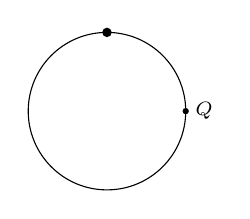
\begin{tikzpicture}[>=stealth,font=\scriptsize]
	\draw (0,0) circle(1);
	\fill (0,1) circle(.06) (1,0)node[right]{\(Q\)} circle(.04);
\end{tikzpicture}
\begin{choices}
	\item 在 \(Q\) 点最大
	\item 在 \(Q\) 点最小
	\item 先减小后增大
	\item 先增大后减小
\end{choices}
\begin{answer}
	C\qquad 提示：\(mgR(1 -\cos\theta) = \frac{1}{2}mv^2\)，\(mg\cos\theta - N = \frac{mv^2}{R}\)，可得:\(N = mg(3\cos\theta - 1)\)

	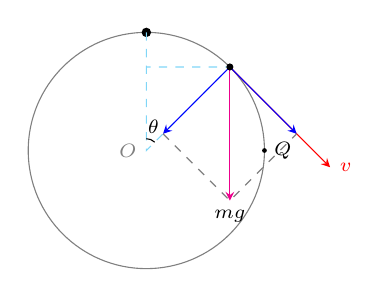
\begin{tikzpicture}[>=stealth,font=\scriptsize,scale=1.5]
		\draw[gray] (0,0)node[left]{\(O\)} circle(1);
		\fill (0,1) circle(.04) (1,0)node[right]{\(Q\)} circle(.02);
		\draw[dashed,cyan!50] (0,1)--(0,0)--(45:1)coordinate(o)--(0,{sqrt(2)/2});
		\draw[->,magenta] (o)--++(0,-{.8*sqrt(2)})coordinate(g)node[below,black]{\(mg\)};
		\draw[->,blue] (o)--++(-135:.8)coordinate(g1);
		\draw[->,red] (o)--++(-45:1.2)node[right]{\(v\)};
		\draw[->,blue] (o)--++(-45:.8)coordinate(g2);
		\draw[gray,dashed] (g1)--(g)--(g2);
		\draw (0,.1) arc(90:45:.1);
		\node at(.06,.2){\(\theta\)};
		\fill (o) circle(.03);
	\end{tikzpicture}
\end{answer}